\documentclass{article}

\usepackage{arxiv}

\usepackage[utf8]{inputenc} % allow utf-8 input
\usepackage[T1]{fontenc}    % use 8-bit T1 fonts
\usepackage{lmodern}        % https://github.com/rstudio/rticles/issues/343
\usepackage{hyperref}       % hyperlinks
\usepackage{url}            % simple URL typesetting
\usepackage{booktabs}       % professional-quality tables
\usepackage{amsfonts}       % blackboard math symbols
\usepackage{nicefrac}       % compact symbols for 1/2, etc.
\usepackage{microtype}      % microtypography
\usepackage{graphicx}

\title{Responsible Repositories}

\author{
    Nathanael Sheehan
   \\
    College of Engineering, Mathematics and Physical Sciences \\
    Exeter University \\
  University of Exeter, St Germans Road, EX4 7HD Exeter, UK \\
  \texttt{\href{mailto:ns651@exeter.ac.uk}{\nolinkurl{ns651@exeter.ac.uk}}} \\
   \And
    Sabina Leonelli
   \\
    EGENIS, Centre For The Study Of Life Sciences \\
    Exeter University \\
  University of Exeter, St Germans Road, EX4 7HD Exeter, UK \\
  \texttt{\href{mailto:s.leonelli@exeter.ac.uk}{\nolinkurl{s.leonelli@exeter.ac.uk}}} \\
  }


% tightlist command for lists without linebreak
\providecommand{\tightlist}{%
  \setlength{\itemsep}{0pt}\setlength{\parskip}{0pt}}


% Pandoc citation processing
\newlength{\cslhangindent}
\setlength{\cslhangindent}{1.5em}
\newlength{\csllabelwidth}
\setlength{\csllabelwidth}{3em}
\newlength{\cslentryspacingunit} % times entry-spacing
\setlength{\cslentryspacingunit}{\parskip}
% for Pandoc 2.8 to 2.10.1
\newenvironment{cslreferences}%
  {}%
  {\par}
% For Pandoc 2.11+
\newenvironment{CSLReferences}[2] % #1 hanging-ident, #2 entry spacing
 {% don't indent paragraphs
  \setlength{\parindent}{0pt}
  % turn on hanging indent if param 1 is 1
  \ifodd #1
  \let\oldpar\par
  \def\par{\hangindent=\cslhangindent\oldpar}
  \fi
  % set entry spacing
  \setlength{\parskip}{#2\cslentryspacingunit}
 }%
 {}
\usepackage{calc}
\newcommand{\CSLBlock}[1]{#1\hfill\break}
\newcommand{\CSLLeftMargin}[1]{\parbox[t]{\csllabelwidth}{#1}}
\newcommand{\CSLRightInline}[1]{\parbox[t]{\linewidth - \csllabelwidth}{#1}\break}
\newcommand{\CSLIndent}[1]{\hspace{\cslhangindent}#1}

\usepackage{booktabs}
\usepackage{longtable}
\usepackage{array}
\usepackage{multirow}
\usepackage{wrapfig}
\usepackage{float}
\usepackage{colortbl}
\usepackage{pdflscape}
\usepackage{tabu}
\usepackage{threeparttable}
\usepackage{threeparttablex}
\usepackage[normalem]{ulem}
\usepackage{makecell}
\usepackage{xcolor}
\begin{document}
\maketitle


\begin{abstract}

\end{abstract}

\keywords{
    SARS-CoV2
   \and
    Open Science
   \and
    Data Governance
  }

\hypertarget{introduction}{%
\section{Introduction}\label{introduction}}

The pandemic demanded rapid, scalable and open access to the latest
research findings, treatments and protocols on the coronavirus. This
shift in research practice - in conjunction with decreasing costs in
data storage - has led to an exponential increase in data repositories
becoming publicly accessible online, as well as a global recognition of
Open Science (OS) principles by the United Nations {[}REF{]}. However,
during the same time, a wider discourse emerged among policy circles and
researchers with concern to the responsibility of repositories reporting
on COVID-19 and related topics, most evidently in relation to the prompt
dissemination of genetic sequencing data from various strains of the
SARS COV-2 virus.

On the 29th of January 2021 the governing board of the European
Bioinformatics Institute (EBI) posted a public letter in Nature calling
for a greater ``openness'' in sharing SARS-CoV-2 genome data, the letter
argued ``to unleash the fast flow of research advances'' the scientific
community must remove all formal barriers which restrict data sharing
and share all genome data to one of a triad of state databases (EBI, The
Gene Bank USA, Japan Gene repo). At the same time, the Global Initiative
on Sharing Avian Influenza Data (GISAID) EpiCov database had just
overtaken the EBI's European COVID-19 Data Portal (C19DP) in the volume
of genome sequences being shared. GISAID was originally established in
2008 to monitor global influenza outbreaks and is now hosted by the
German Institute of Agriculture and the Max Planck institute; the
platforms pivot quickly grew in popularity during the pandemic and
received a number of philanthropic donations from the World Health
Organization, big-pharma and nation states, unlike C19DP, GISAID
requires that users confirm their identity and agree not to republish
the sites genomes without permission from the data provider.

Leonelli (2021) introduces this case study as a clash in ``responsible
research measures,'' pointing out how ``trustworthy and explicitly
non-exploitative conditions for data sharing helps to widen
participation in data sharing,'' in this same line of thought we
stipulate that Trust and Responsibility, or a lack of it, plays a
central role in the success of OS platforms; hence researchers and data
producers alike, must ensure quality and integrity of data when
practicing OS principles in order to demonstrate the quality and
discipline which OS research demands.

The TRUST (Transparency, Responsibility, User Focus, Sustainability, and
Technology) principles put forth a set of guidelines to demonstrate the
trustworthiness of a digital repository to many of the stakeholders
involved, including researchers, community users, funders, developers
and service providers. In an OS context, a number of trustworthiness
certification mechanisms already exist; The Open Archival Information
System (OAIS) provides a recommendation model to provide long-term
preservation and access to digital information {[}REF{]} and the FAIR
principles emphasize a best practice of machine and human re-usability
with data objects. However, Lin et al (2020) argue these frameworks are
not suitable for a broader audience and lack a critical understanding of
the temporal aspects of a data repository, data may enter a system under
a FAIR or OAIS system, however TRUST should not be understood as a
single check box, rather it must regularly audited to ensure the system
ensures trust for the long run (Lin et al 2020). Repository users should
have confidence that data depositors are prompted to provide all
metadata compliant with the community norms, as this greatly enhances
the discoverability and usefulness of the data. Knowing that a
repository verifies the integrity of available data and metadata assures
potential users that the data holdings are more likely to be
interoperable with other relevant datasets. Both depositors and users
must have confidence that the data will remain accessible over time, and
thus can be cited and referenced in scholarly publications. Building on
previous discussions on Epistemic diversity and Open Science, we propose
a novel metric system based on the description of the R principle in
TRUST (Lin et al 2020) to be used in tandem with a qualitative
understanding to interpret the philosophical nuances of differing
implementations of openness.

\hypertarget{methods}{%
\section{Methods}\label{methods}}

\hypertarget{definition}{%
\subsection{Definition}\label{definition}}

Stakeholders of a repository must take responsibility - legally and
ethically- for the data being stored and collected from their user
community. Lin et al (2020) delineates responsibility being demonstrated
as:

\begin{itemize}
\item
  "\emph{Adhering to the designated community's metadata and curation
  standards, along with providing stewardship of the data holdings
  e.g.~technical validation, documentation, quality control,
  authenticity protection, and long-term persistence.}
\item
  \emph{Providing data services e.g.~portal and machine interfaces, data
  download or server-side processing.}
\item
  \emph{Managing the intellectual property rights of data producers, the
  protection of sensitive information resources, and the security of the
  system and its content.}"
\end{itemize}

We classify our reading of responsibility into three distinct modes
which are described by sub classifications metrics. Each metric varies
on a scale from 0-1, where 0 indicates the responsibility classification
is ``not implemented,'' 0.4 indicates the responsibility classification
is ``partially implemented'' and 0.9 indicates the responsibility
classification is ``Sufficiently implemented.'' The total score for each
distinct mode is calculated as a mean weighted average from each of its
sub classifications.

\begin{table}[H]

\caption{\label{tab:fig1}Modes of responsiblity and sub classifcations metrics}
\centering
\begin{tabular}[t]{l|l|l}
\hline
Metadata Responsibility & Service Responsibility & Legal Responsibility\\
\hline
R1.1 Curated Metadata & R2.1 Reliable Data Services & R3.1 Manage IP of Data Producers\\
\hline
R1.2 Techincal Documentation &  & R3.2 Security of System\\
\hline
R1.3 Format Control &  & R3.3 Security of Content\\
\hline
R1.4 Content Control &  & \\
\hline
R1.5 Authenticated Provinence &  & \\
\hline
\end{tabular}
\end{table}

\hypertarget{metadata-responsibility}{%
\subsection{Metadata Responsibility}\label{metadata-responsibility}}

Metadata Responsibility is the largest group of sub-classifications and
focuses on the quality, re-usability and interoperability of data stored
on the repository. \texttt{R1.1\ Sufficient\ Metadata} asserts
repository metadata to conform to a general curation standard whereby
data can be transformed for further discoverability.
\texttt{R1.2\ Technical\ Documentation} requires a closed reading of
each repository `docs,' and evaluates whether the documents provide
clear and useful instructions to successfully interact and use the
platform. \texttt{R1.3\ Format\ Control} concerns a format control test
to ensure that users uploading data have to do so in a standardized
form. \texttt{R1.4\ Content\ Control} asks if user content goes under a
form of peer review to ensure integrity of data producers.
\texttt{R1.5\ Authenticated\ Provinence} checks if there are forms of
authentication to interact with the data respiratory.

\hypertarget{service-responsibility}{%
\subsection{Service Responsibility}\label{service-responsibility}}

Service Responsibility is the smallest group of sub-classifications and
focuses on the tools presented to download and upload data.
\texttt{R2.1\ Reliable\ Data\ Services} tests the range of tools
available to download data from the platform and tests if data can be
downloaded in a range of formats and is machine readable.

\hypertarget{legal-responsibility}{%
\subsection{Legal Responsibility}\label{legal-responsibility}}

Legal Responsibility is a critical component to the R in trust as it
binds the digital and physical world.
\texttt{R3.1\ Manage\ IP\ of\ Data\ Producers} verifies the intellectual
property policy for data producers and the effects this has for users of
the platform. \texttt{R3.2\ Security\ of\ System} studies the
vulnerabilities in infrastructure which uphold the data, the platform
and the various microservices which contribute to the functioning of the
whole system. \texttt{R3.3\ Security\ of\ Content}

\hypertarget{results}{%
\section{Results}\label{results}}

\begin{table}[H]

\caption{\label{tab:fig3}Results}
\centering
\begin{tabular}[t]{l|r|r}
\hline
Metric & GISAID: EpiCov & EBI: Covid-19 Data Platform\\
\hline
R1.1 Sufficent Metadata & 0.4 & 0.9\\
\hline
R1.2 Techincal Documentation & 0.4 & 0.9\\
\hline
R1.3 Format Control & 0.9 & 0.9\\
\hline
R1.4 Content Control & 0.9 & 0.9\\
\hline
R1.5 Authenticated Provinence & 0.9 & 0.0\\
\hline
R2.1 Reliable Data Services & 0.9 & 0.4\\
\hline
R3.1 Manage IP of Data Producers & 0.4 & 0.0\\
\hline
R3.2 Security of System & 0.4 & 0.4\\
\hline
R3.3 Security of Content & 0.9 & 0.0\\
\hline
Total Score & 6.1 & 4.4\\
\hline
\end{tabular}
\end{table}

\hypertarget{discussion}{%
\section{Discussion}\label{discussion}}

\hypertarget{references}{%
\section{References}\label{references}}

\begin{figure}
\centering
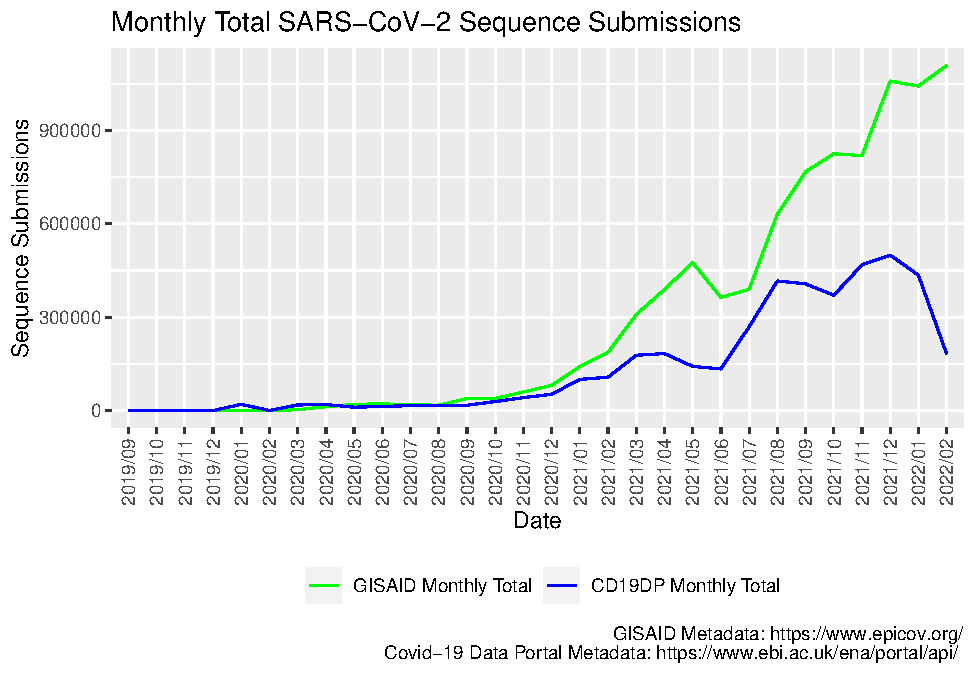
\includegraphics{Report_files/figure-latex/fig2-1.pdf}
\caption{Monthly totals of global SARS-CoV-2 cases sequenced and shared
on the GISAID and Covid-19 Data Platform database until Febuary 22 2022}
\end{figure}

\hypertarget{refs}{}
\begin{CSLReferences}{1}{0}
\leavevmode\hypertarget{ref-pittphilsci19817}{}%
Leonelli, Sabina. 2021. {``Open Science and Epistemic Diversity: Friends
or Foes?''} In. \url{http://philsci-archive.pitt.edu/19817/}.

\end{CSLReferences}

\bibliographystyle{unsrt}
\bibliography{references.bib}


\end{document}
